\باب{موصل، ذوبرق اور  کپیسٹر}
اس باب میں ہم برقی رو اور کثافت برقی رو سے شروع ہو کر بنیادی \اصطلاح{استمراری مساوات}\حاشیہب{continuity equation}  حاصل کریں گے۔اس کے بعد  اوہم کے قانون کی نقطہ شکل  اور اس کی بڑی شکل حاصل کریں گے۔دو اجسام کے جوڑ پر \اصطلاح{سرحدی شرائط}\حاشیہب{boundary conditions} حاصل کرتے ہوئے \اصطلاح{عکس}\حاشیہب{images} کے طریقے کا استعمال دیکھیں گے۔

\اصطلاح{ذوبرق}\حاشیہب{dielectric}  کی \اصطلاح{تقطیب}\حاشیہب{polarization} پر غور کرتے ہوئے  جزو برقی مستقل حاصل کریں گے۔اس کے بعد کپیسٹر پر غور کیا جائے گا۔سادہ شکل و صورت رکھنے والے  کپیسٹر کی قیمتیں حاصل کی جائیں گیں۔ایسا گزشتہ بابوں کے نتائج استعمال کرتے ہوئے کیا جائے گا۔ 

\حصہ{برقی رو اور کثافت برقی رو}
جیسے پانی کے حرکت کو پانی کا بہاو کہتے ہیں،  اسی طرح برقی چارج کے حرکت کو برقی رو کہتے ہیں۔برقی رو کو \عددیء{i} اور \عددیء{I} سے ظاہر کیا جاتا ہے۔برقی رو کی اکائی ایمپیئر \عددیء{(A)} ہے۔کسی نقطے یا سطح سے ایک کولمب چارج فی سیکنڈ کے گزر کو ایک ایمپیئر کہتے ہیں۔یوں
\begin{align}
I=\frac{\dif Q}{\dif t}
\end{align}
لکھا جائے گا۔

ایسی موصل تار جس کی ایک سرے سے دوسری سرے تک موٹائی مسلسل کم ہوتی ہو کے بالکل محور پر برقی چارج محوری سمت میں حرکت کرے گا جبکہ محور سے دور چارج کی حرکت تار کی موٹائی کم یا زیادہ ہونے کی وجہ سے قدرِ ترچھی ہو گی۔یوں اگرچہ تار میں ہر مقام پر برقی رو کی مقدار برابر ہے لیکن برقی رو کی سمتیں مختلف ہو سکتی ہیں۔اسی بنا پر ہم برقی رو کو مقداری تصور کریں گے۔اگر تار کی موٹائی انتہائی کم ہو تب برقی رو سمتیہ مانند ہو گا لیکن ایسی صورت میں بھی ہم اسے مقداری ہی تصور کرتے ہوئے تار کی لمبائی کو سمتیہ لیں گے۔

\اصطلاح{کثافت برقی رو}\فرہنگ{برقی رو!کثافت}\حاشیہب{current density}\فرہنگ{density!current} سے مراد برقی رو فی اکائی مربع سطح \عددیء{(\si{\ampere \per \meter \squared})} ہے اور اسے \عددیء{J} سے ظاہر کیا جاتا ہے۔اگر چھوٹی سطح \عددیء{\Delta S} سے عمودی سمت میں \عددیء{\Delta I} برقی رو گزرے تب
\begin{align}
\Delta I=J_n \Delta S
\end{align}
کے برابر ہو گا۔اگر کثافت برقی رو اور سمتی رقبہ کی سمتیں مختلف ہوں تب
\begin{align}
\Delta I = \kvec{J} \cdot \Delta S
\end{align}
لکھا جائے گا اور پوری سطح سے کُل گزرتی برقی رو تکمل کے ذریعہ حاصل کی جائے گی۔
\begin{align} \label{مساوات_کپیسٹر_برقی_رو_کثافت_کا_سطحی_تکمل_ہے}
I=\int_S \kvec{J} \cdot \dif \kvec{S}
\end{align}
%
\ابتدا{مثال}
شکل \حوالہ{شکل_کپیسٹر_سطح_سے_گزرتی_برقی_رو} میں سیدھی سطح \عددیء{\kvec{S}=2\ax} دکھائی گئی ہے جہاں کثافت برقی رو \عددیء{\kvec{J}=1\ax+1\ay} پائی جاتی ہے۔سطح سے گزرتی برقی رو اور اس کی سمت دریافت کریں۔اگر سطح کی دوسری سمت کو سطح کی سمت لی جائے تب برقی رو کی مقدار اور اس کی سمت کیا ہوں گے۔
\begin{figure}
\centering
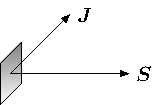
\includegraphics{figCapacitorCurrentFromCurrentDensityDotArea}
\caption{سطح سے گزرتی برقی رو۔}
\label{شکل_کپیسٹر_سطح_سے_گزرتی_برقی_رو}
\end{figure}

حل:چونکہ  یہاں \عددیء{\kvec{J}} مستقل مقدار ہے لہٰذا اسے مساوات \حوالہ{مساوات_کپیسٹر_برقی_رو_کثافت_کا_سطحی_تکمل_ہے} میں تکمل کے باہر لایا جا سکتا ہے اور یوں اس تکمل سے
\begin{align*}
I=\kvec{J} \cdot \kvec{S}= \SI{2}{\ampere}
\end{align*} 
حاصل ہوتا ہے۔برقی رو چونکہ مثبت ہے لہٰذا یہ سطح کی سمت میں ہی سطح سے گزر رہی ہے۔

اگر سطح کی دوسری طرف کو سطح کی سمت لی جائے تب \عددیء{\kvec{S}=-2\ax} لکھا جائے گا اور یوں
\begin{align*}
I=\kvec{J} \cdot \kvec{S}= \SI{-2}{\ampere}
\end{align*} 
حاصل ہو گا۔برقی رو کی مقدار اب بھی دو ایمپیئر ہی ہے البتہ اس کی علامت منفی ہے جس کا مطلب یہ ہے کہ برقی رو سطح کے سمت کی الٹی سمت میں ہے۔یوں اب بھی برقی رو بائیں سے دائیں ہی  گزر رہی ہے۔

\انتہا{مثال}
%

اس مثال سے آپ دیکھ سکتے ہیں کہ \عددیء{\kvec{S}} کی سمت میں برقی رو کو مثبت برقی رو کہا جاتا ہے۔
\begin{figure}
\centering
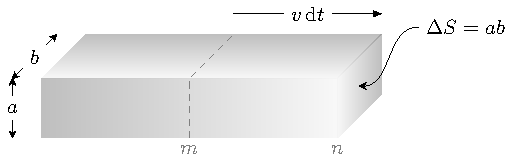
\includegraphics{figCapacitorPointFormOfOhmLaw}
\caption{حرکت کرتے چارج کی رفتار اور کثافت برقی رو۔}
\label{شکل_کپیسٹر_حرکت_کرتا_چارج_اور_کثافت_برقی_رو}
\end{figure}

شکل \حوالہ{شکل_کپیسٹر_حرکت_کرتا_چارج_اور_کثافت_برقی_رو} میں \عددیء{a} اور \عددیء{b} اطراف کی تار میں لمبائی کی سمت میں \عددیء{v} رفتار سے چارج حرکت کر رہا ہے۔شکل میں اس تار کا کچھ حصہ دکھایا گیا ہے۔یوں \عددیء{\dif t} دورانیہ میں چارج \عددیء{v \dif t} فاصلہ طے کرے گا۔اس طرح اس دورانیہ میں \عددیء{m} پر لگائی گئی نقطہ دار لکیر \عددیء{n} پہنچ جائے گی۔آپ دیکھ سکتے ہیں کہ اس دورانیہ میں \عددیء{m} اور \عددیء{n} کے درمیان موجود چارج سطح \عددیء{\Delta S} سے گزر جائے گا۔\عددیء{m} سے \عددیء{n} تک حجم \عددیء{a b v \dif t} کے برابر ہے۔اگر تار میں چارج کی حجمی کثافت \عددیء{\rho_h} ہو تب اس حجم میں  کُل چارج \عددیء{\rho_h a b v \dif t } ہو گا۔یوں برقی رو
\begin{align*}
I=\frac{\Delta Q}{\Delta t}=\frac{\rho_h a b v \dif t}{\dif t}=\rho_h \Delta S v
\end{align*}
لکھتے ہوئے  کثافت برقی رو
\begin{align*}
J=\frac{I}{\Delta S}=\rho_h v
\end{align*}
حاصل ہوتی ہے جس کی سمتی شکل
\begin{align}\label{مساوات_کپیسٹر_کثافت_رو_مساوی_کثافت_چارج_ضرب_رفتار}
\kvec{J}=\rho_h \kvec{v}
\end{align}
ہے۔

یہ مساوات کہتا ہے کہ حجمی چارج کثافت بڑھانے سے کثافت برقی رو اسی نسبت سے بڑھتی ہے۔اسی طرح چارج کی رفتار بڑھانے سے کثافت برقی رو اسی نسبت سے بڑھتی ہے۔یہ ایک عمومی نتیجہ ہے۔یوں سڑک پر زیادہ لوگ گزارنے کا ایک طریقہ انہیں تیز چلنے پر مجبور کرنے سے حاصل کیا جا سکتا ہے۔دوسرا طریقہ یہ ہے کہ انہیں قریب قریب کر دیا جائے۔ 


\حصہ{استمراری مساوات}
قانون بقائے چارج کہتا ہے کہ چارج کو نہ تو پیدا  اور نا ہی اسے ختم کیا جا سکتا ہے، اگرچہ برابر مقدار میں مثبت اور منفی چارج کو ملا کی انہیں ختم کیا جا سکتا ہے اور اسی طرح برابر مقدار میں انہیں پیدا بھی کیا جا سکتا ہے۔

یوں اگر ڈبے میں ایک جانب \عددیء{\SI{+5}{\coulomb}} اور دوسری جانب \عددیء{\SI{-3}{\coulomb}} چارج موجود ہو تو اس ڈبے میں کُل \عددیء{\SI{2}{\coulomb}} چارج ہے۔اگر ہم \عددیء{\SI{+3}{\coulomb}}  کو \عددیء{\SI{-3}{\coulomb}}  کے ساتھ ملا کر ختم کر دیں تب  بھی ڈبے میں کُل \عددیء{\SI{2}{\coulomb}} ہی چارج رہے گا۔

%=================
\ابتدا{مثال}
ایک ڈبہ جس کا حجم \عددیء{\SI{5}{\meter^3}} ہے میں حجمی کثافت چارج \عددیء{\SI{3}{\coulomb \per \meter^3}} ہے۔اس ڈبے سے چارج کی نکاسی ہو رہی ہے۔دو سیکنڈ میں حجمی کثافت چارج \عددیء{\SI{1}{\coulomb \per \meter^3}} رہ جاتی ہے۔ان دو سکینڈوں میں ڈبے سے خارج برقی رو کا تخمینہ لگائیں۔

حل:شروع میں ڈبے میں \عددیء{Q_1=3 \times 5=\SI{15}{\coulomb}} چارج ہے جبکہ دو سیکنڈ بعد اس میں \عددیء{Q_1=1 \times 5=\SI{5}{\coulomb}} رہ جاتا ہے۔یوں دو سیکنڈ میں ڈبے سے \عددیء{\SI{10}{\coulomb}} چارج خارج ہوتا ہے۔اس طرح  ڈبے سے خارج برقی رو \عددیء{\tfrac{10}{2}=\SI{5}{\ampere}} ہے۔اسی کو یوں لکھا جا سکتا ہے۔
\begin{align*}
I=-\frac{\Delta Q}{\Delta t}=-\frac{(5-15)}{2}=\SI{5}{\ampere}
\end{align*}
\انتہا{مثال}
%=======================

اس مثال میں آپ نے دیکھا کہ ڈبے میں \عددیء{\Delta Q} منفی ہونے کی صورت میں خارجی برقی رو کی قیمت مثبت ہوتی ہے۔آئیں اس حقیقت کو بہتر شکل دیں۔

حجم کو مکمل طور پر گھیرتی سطح کو بند سطح کہتے ہیں۔کسی بھی مقام پر ایسی سطح کی سمت سطح کے عمودی باہر کو ہوتی ہے۔مساوات \حوالہ{مساوات_کپیسٹر_برقی_رو_کثافت_کا_سطحی_تکمل_ہے} کے تحت برقی رو کو کثافت برقی رو کے سطحی تکمل سے بھی حاصل کیا جا سکتا ہے۔یوں
\begin{align}\label{مساوات_کپیسٹر_استمراری_مساوات_تکمل_شکل}
I=\oint_S \kvec{J} \cdot \dif \kvec{S}=-\frac{\dif Q}{\dif t}
\end{align}
لکھا جا سکتا ہے جہاں حجم کی سطح بند سطح ہونے کی بنا پر بند تکمل کی علامت استعمال کی گئی ہے اور \عددیء{Q} حجم میں کل چارج ہے۔

مساوات \حوالہ{مساوات_کپیسٹر_استمراری_مساوات_تکمل_شکل} \اصطلاح{استمراری مساوات}\فرہنگ{استمراری مساوات}\حاشیہب{continuity equation}\فرہنگ{continuity equation} کی تکمل شکل ہے۔آئیں اب اس کی نقطہ شکل حاصل کریں۔

مسئلہ پھیلاو کو صفحہ \حوالہصفحہ{مساوات_گاوس_مسئلہ_پھیلاو_تکمل_شکل} پر مساوات \حوالہ{مساوات_گاوس_مسئلہ_پھیلاو_تکمل_شکل} میں بیان کیا گیا ہے۔مسئلہ پھیلاو کسی بھی سمتی تفاعل کے لئے درست ہے لہٰذا اسے استعمال کرتے ہوئے مساوات \حوالہ{مساوات_کپیسٹر_استمراری_مساوات_تکمل_شکل} میں بند سطحی تکمل کو حجمی تکمل میں تبدیل کرتے ہیں۔
\begin{align*}
\oint_S \kvec{J} \cdot \dif \kvec{S}=\int_h (\nabla \cdot \kvec{J}) \dif h
\end{align*}
اگر حجم میں حجمی کثافت چارج \عددیء{\rho_h} ہو تب اس میں کل چارج
\begin{align*}
Q=\int_h \rho_h \dif h
\end{align*}
ہو گا۔ان دو نتائج کو استعمال کرتے ہوئے
\begin{align*}
\int_h (\nabla \cdot \kvec{J}) \dif h=-\frac{\dif}{\dif t} \int_h \rho_h \dif h
\end{align*}
لکھا جا سکتا ہے۔اس مساوات میں \عددیء{\tfrac{\dif}{\dif t}} دو متغیرات پر لاگو ہو گا۔یہ متغیرات تکمل کے اندر حجمی چارج کثافت \عددیء{\rho_h} اور حجم \عددیء{h} ہے۔

آپ جانتے ہیں کہ دو متغیرات کے تفرق کو جزوی تفرق کی شکل میں
\begin{align*}
\frac{\dif (uv)}{\dif t}=\frac{\partial u}{\partial t} v+ u  \frac{\partial v}{\partial t}
\end{align*}
لکھا جا سکتا ہے جہاں \عددیء{v} کو مستقل رکھتے ہوئے \عددیء{\tfrac{\partial u}{\partial t}} اور \عددیء{u} کو مستقل رکھتے ہوئے \عددیء{\tfrac{\partial v}{\partial t}} حاصل کیا جاتا ہے۔

اگر ہم یہ شرط لاگو کریں کہ حجم کی سطح تبدیل نہیں ہو گی تب حجم بھی تبدیل نہیں ہو گا اور یوں \عددیء{\tfrac{\dif}{\dif t}} کو جزوی تفرق میں تبدیل کرتے ہوئے تکمل کے اندر لکھتے ہوئے
\begin{align*}
\int_h (\nabla \cdot \kvec{J}) \dif h=\int_h -\frac{\partial \rho_h}{\partial t} \dif h
\end{align*}
حاصل ہوتا ہے۔یہ مساوات ہر ممکنہ حجم کے لئے درست ہے لہٰذا یہ نہایت چھوٹی حجم کے لئے بھی درست ہے۔نہایت چھوٹی حجم \عددیء{\dif h} کے لئے تکمل
\begin{align*}
 (\nabla \cdot \kvec{J}) \dif h= -\frac{\partial \rho_h}{\partial t} \dif h
\end{align*}
ہی ہے جس سے
\begin{align}\label{مساوات_کپیسٹر_استمراری_مساوات_نقطہ_شکل}
\nabla \cdot \kvec{J}=-\frac{\partial \rho_h}{\partial t}
\end{align}
حاصل ہوتا ہے۔مساوات \حوالہ{مساوات_کپیسٹر_استمراری_مساوات_نقطہ_شکل} استمراری مساوات کی نقطہ شکل ہے۔

پھیلاو کی تعریف کو ذہن میں رکھتے ہوئے آپ دیکھ سکتے ہیں کہ مساوات \حوالہ{مساوات_کپیسٹر_استمراری_مساوات_نقطہ_شکل} کہتا ہے کہ ہر نقطے پر چھوٹی سی حجم سے فی سیکنڈ چارج کا اخراج، یعنی برقی رو، فی اکائی حجم مساوی ہے چارج کے گھٹاو فی سیکنڈ فی اکائی حجم۔ 


\حصہ{موصل}
غیر چارج شدہ موصل میں منفی الیکٹران اور مثبت ساکن ایٹموں کی تعداد برابر ہوتی ہے البتہ اس میں برقی رو آزاد الیکٹران کے حرکت سے پیدا ہوتا ہے۔موصل میں الیکٹران آزادی سے بے ترتیب حرکت کرتا رہتا ہے۔یہ حرکت کرتا ہوا لمحہ بہ لمحہ ساکن ایٹم سے ٹکراتا ہے اور ہر ٹکر سے اس کے حرکت کی سمت تبدیل ہو جاتی ہے۔یوں ایسے الیکٹران کی اوسط رفتار صفر کے برابر ہوتی ہے۔آئیں دیکھیں کہ برقی میدان کے موجودگی میں کیا ہوتا ہے۔

برقی میدان \عددیء{\kvec{E}} میں الیکٹران پر قوت
\begin{align}
\kvec{F}=-e\kvec{E}
\end{align}
عمل کرے گی جہاں الیکٹران کا چارج \عددیء{-e} ہے۔ الیکٹران کی رفتار اس قوت کی وجہ سے  اسراع کے ساتھ قوت کی سمت میں بڑھنے شروع ہو جائے گی۔یوں بلا ترتیب رفتار  کے ساتھ ساتھ قوت کے سمت میں الیکٹران رفتار پکڑے گا۔موصل میں پائے جانے والا الیکٹران جلد کسی ایٹم سے ٹکرا جاتا ہے اور یوں اس کی سمت تبدیل ہو جاتی ہے۔جس لمحہ  الیکٹران کسی ایٹم سے ٹکراتا ہے اگر لاگو میدان کو صفر کر دیا جائے تو الیکٹران دوبارہ بلا ترتیب حرکت کرتا رہے گا اور اس کی اوسط رفتار دوبارہ صفر ہی ہو گی،  البتہ اس کی رفتار اب پہلے سے زیادہ ہو گی۔اگر الیکٹران ایٹم سے نہ ٹکراتا تب برقی میدان صفر کرنے کے بعد یہ برقرار قوت کی سمت میں حاصل کردہ رفتار سے حرکت کرتا رہتا۔یوں آپ دیکھ سکتے ہیں کہ ہر ٹکر سے الیکٹران کی اوسط رفتار صفر ہو جاتی ہے۔
اس طرح ہم دیکھتے ہیں کہ  \عددیء{\kvec{E}} کے موجودگی میں موصل میں الیکٹران کی رفتار مسلسل نہیں بڑھتی بلکہ یہ قوت کی سمت میں اوسط رفتار \عددیء{\kvec{v}_d} حاصل کرتا ہے اور جیسے ہی میدان صفر کر دیا جائے الیکٹران کی اوسط رفتار بھی صفر ہو جاتی ہے۔\عددیء{\kvec{v}_d} کو \اصطلاح{رفتار بہاو}\فرہنگ{رفتار بہاو}\حاشیہب{drift velocity}\فرہنگ{drift velocity} کہتے ہیں۔رفتار بہاو کا دارومدار \عددیء{\kvec{E}} کی قیمت پر ہے لہٰذا ہم
\begin{align}\label{مساوات_کپیسٹر_رفتار_بہاو}
\kvec{v}_d=-\mu_e \kvec{E}
\end{align}
لکھ سکتے ہیں جہاں مساوات کے مستقل \عددیء{\mu_e} کو الیکٹران کی \اصطلاح{حرکت پذیری}\فرہنگ{حرکت پذیری!الیکٹران}\حاشیہب{mobility}\فرہنگ{mobility!electron} کہتے ہیں۔حرکت پذیری کی مقدار مثبت ہے ۔چونکہ \عددیء{\kvec{v}_d} کو میٹر فی سیکنڈ اور \عددیء{\kvec{E}} کو وولٹ فی میٹر میں ناپا جاتا ہے لہٰذا حرکت پذیری کو \عددیء{\si{\meter \squared \per \volt \per \second}} میں ناپا جائے گا۔

مساوات \حوالہ{مساوات_کپیسٹر_رفتار_بہاو} کو صفحہ \حوالہصفحہ{مساوات_کپیسٹر_کثافت_رو_مساوی_کثافت_چارج_ضرب_رفتار} پر دئے مساوات \حوالہ{مساوات_کپیسٹر_کثافت_رو_مساوی_کثافت_چارج_ضرب_رفتار} میں پر کرتے ہوئے
\begin{align}
\kvec{J}=-\rho_e \mu_e \kvec{E}
\end{align}
حاصل ہوتا ہے جہاں موصل میں آزاد الیکٹران کی حجمی چارج کثافت کو \عددیء{\rho_e} لکھا گیا ہے۔\عددیء{\rho_e} منفی مقدار ہے۔یاد رہے کہ غیر چارج شدہ موصل میں حجمی کثافت چارج صفر کے برابر ہے چونکہ اس میں منفی الیکٹران  اور مثبت ایٹم کے چارج برابر ہوتے ہیں۔اس مساوات کو عموماً
\begin{align}\label{مساوات_کپیسٹر-اوہم_قانون_نقطہ_شکل}
\kvec{J}=\sigma \kvec{E}
\end{align}
لکھا جاتا ہے جو اوہم کے قانون\فرہنگ{قانون!اوہم}\فرہنگ{Ohm's law} کی نقطہ شکل ہے اور جہاں
\begin{align}\label{مساوات_کپیسٹر_موصلیت_تعریف}
\sigma=-\rho_e \mu_e
\end{align}
لکھا گیا ہے۔\عددیء{\sigma} کو \اصطلاح{موصلیت کا مستقل}\فرہنگ{موصلیت!مستقل}\حاشیہب{conductivity}\فرہنگ{conductivity} کہتے ہیں اور اس کی اکائی\حاشیہد{یہ اکائی جرمنی کے جناب ارنسٹ ورنر وان سیمنز (1816-1892) کے نام ہے جنہوں نے موجودہ سیمنز کمپنی کا بنیاد رکھا۔} سیمنز فی میٹر \عددیء{\si{\siemens \per \meter}} ہے۔سیمنز کو بڑے \عددیء{\si{\siemens}} سے  جبکہ سیکنڈ کو چھوٹے \عددیء{\second} سے ظاہر کیا جاتا ہے۔امید کی جاتی ہے کہ آپ ان میں غلطی نہیں کریں گے۔ اس کتاب کے آخر میں صفحہ  \حوالہصفحہ{جدول_جدول_موصلیت_کے_مستقل} پر جدول \حوالہ{جدول_جدول_موصلیت_کے_مستقل} میں کئی موصل اور غیر موصل اشیاء کی موصلیت پیش کی گئی ہیں۔
%================
\ابتدا{مثال}
تانبے\فرہنگ{تانبا}\حاشیہب{copper}\فرہنگ{copper} کی موصلیت کے مستقل  کی قیمت \عددیء{\SI{5.8e7}{\siemens \per \meter}} ہے جبکہ اس کی کمیتی کثافت \عددیء{\SI{8940}{\kilogram \per \meter^3}} اور ایٹمی کمیت \عددیء{\SI{63.5}{\gram}} ہیں۔اگر ہر ایٹم ایک عدد الیکٹران آزاد کرتا ہو تب تانبے میں الیکٹران کی حرکت پذیری حاصل کریں۔\عددیء{E=\SI{0.1}{\volt \per \meter}} کی صورت میں الیکٹران کا رفتار بہاو حاصل کریں۔

حل:ایٹمی کمیت \عددیء{\num{6.023e23}} یعنی ایک مول\حاشیہب{mole} ایٹم کی کمیت کو کہتے ہیں۔چونکہ ایک مربع میٹر میں \عددیء{\SI{8940}{\kilogram}} ہیں لہٰذا ایک مربع میٹر میں
\begin{align*}
\frac{8940 \times 6.023 \times 10^{23}}{0.0635}=8.48 \times 10^{28}
\end{align*} 
ایٹم پائیں جائیں گے۔ہر ایٹم ایک الیکٹران آزاد کرتا ہے لہٰذا \عددیء{\SI{0.1}{\nano \meter}} اطراف کے مربع میں اوسطاً \عددیء{0.848} یعنی تقریباً ایک عدد آزاد الیکٹران پایا جائے گا۔ اس طرح  ایک مربع میٹر میں کل آزاد الیکٹران چارج یعنی حجمی آزاد چارج کثافت
\begin{align*}
\rho_e=-1.6 \times 10^{-19} \times 8.48 \times 10^{28}=\SI{-1.36e10}{\coulomb \per \meter^3}
\end{align*}
ہو گی۔اس طرح مساوات \حوالہ{مساوات_کپیسٹر_موصلیت_تعریف} کی مدد سے
\begin{align*}
\mu_e=-\frac{\sigma}{\rho_e}=\frac{5.8 \times 10^7}{-1.36 \times 10^{10}}=\SI{0.00427}{\meter \squared \per \volt \per \second}
\end{align*}
حاصل ہوتا ہے جہاں \عددیء{\SI{0.00427}{\meter \squared \siemens \per \coulomb}} کو \عددیء{\SI{0.00427}{\meter \squared \per \volt \per \second}} لکھا گیا ہے۔آپ تسلی کر سکتے ہیں کہ یہ برابر مقدار ہیں۔اب مساوات  \حوالہ{مساوات_کپیسٹر_رفتار_بہاو} استعمال کرتے ہوئے الیکٹران کی رفتار بہاو 
\begin{align*}
v_d = -0.00427 \times 0.1=\SI{-0.000427}{\meter \per \second}
\end{align*}
حاصل ہوتی ہے۔منفی رفتار کا مطلب ہے کہ الیکٹران \عددیء{\kvec{E}} کے الٹ سمت حرکت کر رہا ہے۔اس رفتار\حاشیہد{کھودا پہاڑ، نکلا چوہا۔آزاد الیکٹران تو کچھوے سے بھی آہستہ چلتا ہے۔} سے الیکٹران ایک کلو میٹر کا فاصلہ ستائیس دن و رات چل کر طے کرے گا۔ 
\انتہا{مثال}
%=============

مندرجہ بالا مثال میں بتلایا گیا کہ تانبے کا ہر ایٹم ایک عدد الیکٹران آزاد کرتا ہے۔اس حقیقت کو یوں سمجھا جا سکتا ہے کہ تانبے کا ایٹمی عدد \عددیء{29}ہے۔ایٹم کے کسی بھی مدار میں  \عددیء{2 n^2}  الیکٹران ہو سکتے ہیں جہاں پہلے مدار کے لئے \عددیء{n=1}، دوسرے مدار کے لئے \عددیء{n=2} وغیرہ لیا جاتا ہے۔یوں اس کے پہلے مدار میں \عددیء{2}، دوسرے مدار میں \عددیء{8}، تیسرے مدار میں \عددیء{18} اور آخری مدار\حاشیہد{چوتھے مدار میں \عددیء{32} الیکٹران ممکن ہیں لیکن تانبے کے ایٹم میں اس مدار کے لئے صرف ایک عدد الیکٹران بچتا ہے۔} میں \عددیء{1} الیکٹران ہو گا۔ایٹم آخری مدار میں واحد الیکٹران کو آزاد کرتا ہے۔آئیں اب بڑی شکل میں اوہم کا قانون حاصل کریں۔ 
\begin{figure}
\centering
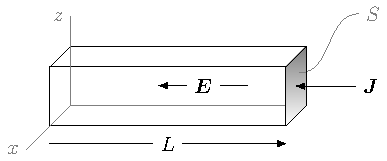
\includegraphics{figCapacitorOhmLawFromPointForm}
\caption{اوہم کے قانون کی بڑی شکل}
\label{شکل_کپیسٹر_اوہم_قانون_بڑی_شکل}
\end{figure}

شکل \حوالہ{شکل_کپیسٹر_اوہم_قانون_بڑی_شکل} میں  موصل سلاخ دکھایا گیا ہے جس کی لمبائی \عددیء{L} اور  رقبہ عمودی تراش \عددیء{S} ہیں۔سلاخ کو \عددیء{\ay} سمت میں لیٹا تصور کریں۔سلاخ میں لمبائی کی سمت میں مستقل اور یکساں برقی میدان \عددیء{\kvec{E}=-E\ay}  اور کثافت برقی رو \عددیء{\kvec{J}=-J\ay} پائے جاتے ہیں۔یوں اگر سلاخ کا بایاں سرا برقی زمین تصور کیا جائے تب اس کے دائیں سرے پر برقی دباو کو صفحہ \حوالہصفحہ{مساوات_توانائی_برقی_دباو_تعریف} پر دئے مساوات \حوالہ{مساوات_توانائی_برقی_دباو_تعریف} سے یوں
\begin{align*}
V= -\int_0^L \kvec{E} \cdot \dif \kvec{L}=\int_0^L E \ay \cdot \dif  y \ay=\int_0^L E \dif y=E\int_0^L \dif y=EL
\end{align*}
حاصل کرتے ہیں۔رقبہ عمودی تراش کو شکل میں گہرے رنگ سے اجاگر کیا گیا ہے۔سمتی رقبہ عمودی تراش بند سطح نہیں ہے لہٰذا اس کے دو ممکنہ رخ ہیں۔سلاخ کے دائیں سرے سے داخل برقی رو حاصل کرنے کی غرض سے رقبہ عمودی تراش کو \عددیء{\kvec{S}=-S\ay} لکھتے ہیں۔یوں دائیں سرے سے داخل برقی رو کی مقدار مثبت ہو گی۔برقی رو
\begin{align*}
I=\int_S \kvec{J} \cdot \dif \kvec{S}=JS
\end{align*}
حاصل ہوتی ہے۔ان معلومات کو شکل \حوالہ{مساوات_کپیسٹر-اوہم_قانون_نقطہ_شکل} میں پُر کرتے ہوئے
\begin{align*}
\frac{I}{S}=\sigma \frac{V}{L}
\end{align*}
  یا
\begin{align*}
V=I \frac{L}{\sigma S}
\end{align*}
حاصل ہوتا ہے جہاں
\begin{align}\label{مساوات_کپیسٹر_سلاخ_کی_مزاحمت}
R= \frac{L}{\sigma S}
\end{align}
کو مزاحمت لکھتے ہوئے
\begin{align}\label{مساوات_کپیسٹر_اوہم_قانون_بڑی_شکل}
V=IR
\end{align}
حاصل ہوتا ہے جو اوہم کے قانون\فرہنگ{اوہم!قانون}\فرہنگ{ohm's law} کی جانی پہچانی شکل ہے۔

مساوات \حوالہ{مساوات_کپیسٹر_سلاخ_کی_مزاحمت} یکساں رقبہ عمودی تراش رکھنے والے موصل سلاخ کی \اصطلاح{مزاحمت}\فرہنگ{مزاحمت}\حاشیہب{resistance}\فرہنگ{resistance} دیتا ہے جہاں مزاحمت کی اکائی \اصطلاح{اوہم}\فرہنگ{اوہم}\حاشیہب{ohm}\فرہنگ{ohm} ہے جسے \عددیء{\si{\ohm}} سے ظاہر کیا جاتا ہے۔یکساں رقبہ عمودی تراش کے سلاخ میں برقی میدان یکساں ہوتا ہے۔اگر سلاخ کا رقبہ عمودی تراش یکساں نہ ہو تب اس میں برقی میدان بھی یکساں نہ ہو گا اور ایسی صورت میں مساوات \حوالہ{مساوات_کپیسٹر_سلاخ_کی_مزاحمت} استعمال نہیں کیا جا سکتا البتہ ایسی صورت میں بھی مزاحمت کو مساوات \حوالہ{مساوات_کپیسٹر_اوہم_قانون_بڑی_شکل} کی مدد سے برقی دباو فی اکائی برقی رو سے بیان کیا جاتا ہے۔یوں مساوات \حوالہ{مساوات_توانائی_برقی_دباو_تعریف} اور مساوات \حوالہ{مساوات_کپیسٹر_برقی_رو_کثافت_کا_سطحی_تکمل_ہے} استعمال کرتے ہوئے سلاخ کے  \عددیء{b} سے \عددیء{a} سرے تک مزاحمت
\begin{align}\label{مساوات_کپیسٹر_مزاحمت_کی_عمومی_مساوات}
R=\frac{V}{I}=\frac{-\int \limits_b^a \kvec{E} \cdot \dif \kvec{L}}{\int \limits_S \kvec{J} \cdot \dif \kvec{S}}=\frac{-\int \limits_b^a \kvec{E} \cdot \dif \kvec{L}}{\int \limits_S \sigma \kvec{E} \cdot \dif \kvec{S}}
\end{align} 
سے حاصل ہو گی جہاں برقی رو سلاخ کے مثبت برقی دباو والے سرے سے سلاخ میں داخل ہوتے برقی رو کو کہتے ہیں۔یوں مندرجہ بالا مساوات میں سطحی تکمل سلاخ کے مثبت سرے پر حاصل کیا جائے گا جہاں سطح عمودی تراش کی سمت سلاخ کی جانب لی جائے گی۔
%=============
\ابتدا{مثال}
تانبے کی ایک کلو میٹر لمبی اور تین ملی میٹر رداس کے تار کی مزاحمت حاصل کریں۔

حل:یہاں \عددیء{L=\SI{1000}{\meter}} جبکہ \عددیء{S=\pi r^2=\SI{2.83e-7}{\meter \squared}} اور \عددیء{\sigma=5.8\times 10^7} ہے لہٰذا
\begin{align*}
R=\frac{1000}{5.8\times 10^7 \times 2.83 \times 10^{-7}}=\SI{0.61}{\ohm}
\end{align*}
حاصل ہوتا ہے۔
\انتہا{مثال}

%=============
\ابتدا{مشق}
المونیم میں کثافت برقی رو مندرجہ ذیل صورتوں میں حاصل کریں۔( الف) برقی میدان کی شدت \عددیء{\SI{50}{\milli \volt \per \meter}} ہے۔ (ب) آزاد الیکٹران کی رفتار بہاو \عددیء{\SI{0.12}{\milli \meter \per \second}} ہے۔ (پ) ایک ملی میٹر موٹی تار جس میں \عددیء{\SI{2}{\ampere}} برقی رو گزر رہی ہے۔

جوابات:\عددیء{\SI{1.91}{\mega \ampere \per \meter \squared}}،  \عددیء{\SI{3.82}{\mega \ampere \per \meter \squared}} اور \عددیء{\SI{2.55}{\mega \ampere \per \meter \squared}}
\انتہا{مشق}
%===============

\حصہ{موصل کے خصوصیات اور سرحدی شرائط}
غیر چارج شدہ موصل میں کُل آزاد الیکٹران اور مثبت ایٹم برابر تعداد میں پائے جاتے ہیں۔یوں اس میں برقی میدان صفر کے برابر ہوتا ہے۔فرض کریں کہ غیر چارج شدہ موصل کے اندر کسی طرح چند الیکٹران نمودار ہو جاتے ہیں۔یہ الیکٹران برقی میدان \عددیء{\kvec{E}} پیدا کریں گے جس کی وجہ سے  موصل میں آزاد الیکٹران  موصل کے سطح کی جانب چل پڑیں گے۔سطح کے باہر غیر موصل خلاء پائی جاتی ہے جس میں الیکٹران حرکت نہیں کر سکتے لہٰذا الیکٹران موصل کے سطح پر پہنچ کر رک جائیں گے۔موصل میں نمودار ہونے والے الیکٹران کے برابر تعداد میں الیکٹران موصل کے سطح پر منتقل ہوں گے جس کے بعد موصل میں دوبارہ منفی الیکٹران اور مثبت ایٹموں کی تعداد برابر ہو جائے گی اور یہ غیر چارج شدہ صورت اختیار کر لے گا۔

آپ نے دیکھا کہ اضافی  چارج موصل میں زیادہ دیر نہیں رہ سکتا اور یہ جلد  سطح پر منتقل ہو جاتا ہے۔یوں اضافی چارج  موصل  کے سطح پر بیرونی جانب چمٹا رہتا ہے۔یہ موصل کی پہلی اہم خاصیت ہے۔

موصل کی دوسری خاصیت \اصطلاح{برقی سکون}\فرہنگ{برقی سکون}\حاشیہب{electrostatic}\فرہنگ{electrostatic} کی حالت کے لئے بیان کرتے ہیں۔برقی سکون سے مراد ایسی صورت ہے جب چارج حرکت نہ کر رہا ہو یعنی جب برقی رو صفر کے برابر ہو۔برقی سکون کی حالت میں موصل کے اندر ساکن برقی میدان صفر رہتا ہے۔اگر ایسا نہ ہوتا تو میدان کی وجہ سے اس میں آزاد الیکٹران حرکت کر کے برقی رو کو جنم دیتے جو غیر ساکن حالت ہے۔

یوں برقی سکون کی حالت میں موصل کے اندر اضافی چارج اور برقی میدان دونوں صفر کے برابر ہوتے ہیں البتہ اس کے سطح پر بیرونی جانب چارج پایا جا سکتا ہے۔آئیں دیکھیں کہ سطح پر پائے جانے والا چارج موصل کے باہر کس قسم کا برقی میدان پیدا کرتا ہے۔

موصل کے سطح پر چارج، موصل کے باہر برقی میدان پیدا کرتا ہے۔سطح پر کسی بھی نقطے پر ایسے میدان کو دو اجزاء کے مجموعے کی شکل میں لکھا جا سکتا ہے۔پہلا جزو سطح کے متوازی اور دوسرا جزو سطح کے عمودی رکھتے ہوئے ہم دیکھتے ہیں کہ سطح کے متوازی جزو صفر ہو گا۔اگر ایسا نہ ہو تو اس میدان کی وجہ سے سطح پر پائے جانے والے آزاد الیکٹران حرکت میں آئیں گے جو غیر ساکن حالت ہو گی۔یوں ہم
\begin{align}
E_{\textup{متوازی}}=0
\end{align}
لکھ سکتے ہیں۔سطح پر عمودی برقی میدان گاوس کے قانون کی مدد سے حاصل کیا جا سکتا ہے جو کہتا ہے کہ کسی بھی بند سطح سے کُل برقی بہاو کا اخراج، سطح میں گھیرے چارج کے برابر ہوتا ہے۔چونکہ سطح پر متوازی برقی میدان صفر ہے اور موصل کے اندر بھی برقی میدان صفر ہے لہٰذا سطح پر چارج سے برقی بہاو کا اخراج صرف عمودی سمت میں ہو سکتا ہے۔یوں \عددیء{\Delta S} سطح سے عمودی اخراج \عددیء{D \Delta S} اسی سطح پر چار \عددیء{\rho_S \Delta S} کے برابر ہو گا جس سے
\begin{align}
D_{\textup{عمودی}}=\rho_S
\end{align} 
حاصل ہوتا ہے۔آئیں اسی بحث کو بہتر جامہ پہنائیں۔

\begin{figure}
\centering
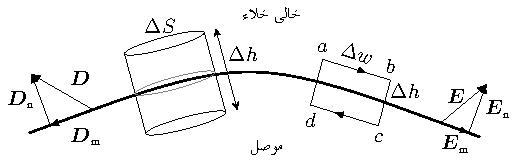
\includegraphics{figCapacitorElectricFieldConductorAirBoundaryCondition}
\caption{موصل اور خلاء کے سرحد پر برقی شرائط۔}
\label{شکل_کپیسٹر_موصل_خلاء_برقی_شرائط}
\end{figure}

شکل \حوالہ{شکل_کپیسٹر_موصل_خلاء_برقی_شرائط} میں موصل اور خالی خلاء کے درمیان سرحد موٹی لکیر سے دکھایا گیا ہے۔اس سرحد پر خلاء کی جانب \عددیء{\kvec{E}} اور \عددیء{\kvec{D}} دکھائے گئے ہیں۔موصل کے اندر \عددیء{\kvec{E}} اور \عددیء{\kvec{D}} دونوں صفر کے برابر ہیں۔خلاء میں \عددیء{\kvec{E}} کو \عددیء{\kvec{E}_\textup{متوازی}} اور \عددیء{\kvec{E}_\textup{عمودی}} کے مجموعے کے طور پر بھی دکھایا گیا ہے جو بالترتیب سرحد کے متوازی اور عمودی \عددیء{\kvec{E}} کے  اجزاء ہیں۔سرحد پر \عددیء{abcd}  مستطیل بنایا گیا ہے جہاں \عددیء{ab} اور \عددیء{cd} سرحد کے متوازی جبکہ \عددیء{bc} اور \عددیء{da} سرحد کے عمودی ہیں۔\عددیء{ab} خالی خلاء میں ہے جبکہ \عددیء{cd} موصل میں ہے۔\عددیء{ab} اور \عددیء{cd} کی لمبائیاں \عددیء{\Delta w} ہیں جبکہ \عددیء{bc} اور \عددیء{da} کی لمبائیاں \عددیء{\Delta h} ہے۔صفحہ \حوالہصفحہ{مساوات_توانائی_بند_راستا} پر دئے مساوات \حوالہ{مساوات_توانائی_بند_راستا} 
\begin{align*}
\oint \kvec{E} \cdot \dif \kvec{L}=0
\end{align*}
کو \عددیء{abcd} پر  استعمال کرتے ہیں۔  
